% ReScience C article content. Every simulated number is a macro from
% ../../paper/results.tex, written by scripts/make_figures.py from data/.

\section*{Introduction}
Bozic et al.\ \cite{bozic2013} modelled the evolution of resistance in metastatic melanoma
lesions treated with targeted therapy. A lesion grows as a multitype birth--death process
from one sensitive cell; resistance to each drug arises by point mutation. From this model
the authors derived closed-form probabilities that resistance is present when treatment
starts and that a lesion is eradicated by one or two drugs (their equation~1), checked
them against simulations, and drew clinical conclusions: a single mutation conferring
cross-resistance to both drugs makes dual therapy fail in most large lesions, combinations
must be given simultaneously rather than sequentially, and patients with a high tumour
burden need three drugs. We re-implemented the model from the paper and its Materials and
methods only (no code was published with the article) and compared our simulations with
its analytic results (Figure~3), its patient-level predictions (Table~1), its simulations
with a cost of resistance (Table~2) and its comparison of sequential and simultaneous
therapy (Figure~5).

\section*{Methods}
\paragraph{Model.} As in \cite{bozic2013}: cell types 00, 10, 01, 11 (1 = resistant to drug
1 or drug 2). Before treatment every cell divides at rate $b$ and dies at rate $d$; the
offspring of a 00 cell is of type 10, 01 or 11 with probabilities $un_1$, $un_2$, $un_{12}$,
that of a 10 cell is 11 with probability $u(n_2+n_{12})$, and symmetrically for 01. The lesion
grows from one sensitive cell until it has $M$ cells; treatment then starts, during which
cells sensitive to at least one drug in use divide at $b'$ and die at $d'$, while fully
resistant cells keep $b$ and $d$. Parameters of Figure~3: $b=0.14$, $d=0.13$, $d'=0.17$,
$b'=b$ per day, $u=10^{-9}$, $n_1=n_2=50$, $n_{12}\in\{0,1,2\}$; for monotherapy, the types
sensitive to drug~1 (00, 01) are treated.

\paragraph{Simulation.} Like the authors, we use a hybrid scheme: a cell type with fewer than
$K=1000$ cells evolves stochastically, larger types deterministically, and mutants of the
large types arise as Poisson events. Small types are advanced in steps of $\Delta t=0.1$~day
with Poisson numbers of births, deaths and mutant offspring (tau-leaping, $b\Delta t=0.014$);
an exact option simulates them event by event (Gillespie), as the authors did. A lesion whose
founding lineage dies out before reaching $M$ is restarted. After treatment starts, a lesion
is eradicated when no cell is left and has failed when a resistant type reaches $10^5$ cells.
Each lesion has its own random stream (xoshiro256** \cite{blackman2021}, seeded from the run
seed and the lesion index), so results do not depend on the number of threads. The code is
C++ with OpenMP, driven from Python.

\paragraph{Extensions used by the paper.} \emph{Cost of resistance} (Table~2): a type with $k$
resistance mutations has birth rate $(b-d)(1-c)^k+d$, with $d=b-0.01$ and $d'=b+0.03$. A cell
made fully resistant by the single cross-resistance mutation carries one mutation and pays the
cost once; one made resistant by two mutations pays it twice. \emph{Sequential therapy}
(Figure~5): drug~1 until relapse, defined as the lesion growing back to $M$ cells after having
shrunk below it, then drug~2. \emph{Division-suppressing therapy}: $b'=0.10$, $d'=0.13$.

\paragraph{Comparison.} Probabilities are compared with Wilson 95\,\% intervals
\cite{wilson1927}. The formulas of \cite{bozic2013} were transcribed from the article's
MathML. Patient lesion sizes come from its Supplementary file~2 (volume = long $\times$
short$^2$/2~cm$^3$, $10^9$ cells/cm$^3$).

\section*{Results}

\paragraph{Equation 1 (Figure 3).} Equation~1 lies inside the 95\,\% interval of our
simulation at \BozicInside{} of \BozicPoints{} points (\BozicLesions{} lesions each; largest
absolute difference \BozicMaxDiff{}; Figure~\ref{fig:erad}). The central result is
reproduced: with one cross-resistance mutation, the probability of eradicating a lesion of
$10^9$ cells falls from \BozicNoCross{} to \BozicOneCross{}.

\begin{figure}[htbp]
\centering
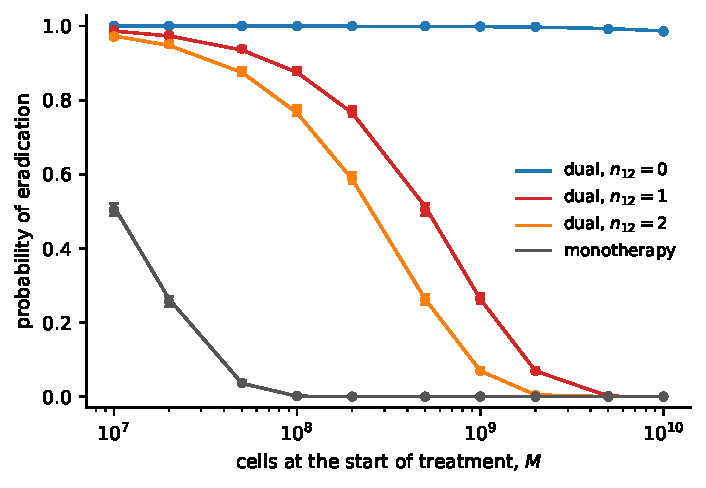
\includegraphics[width=0.75\linewidth]{../../figures/bozic_eradication.pdf}
\caption{Probability of eradicating a lesion of $M$ cells (parameters of Figure~3 of
\cite{bozic2013}). Points: simulation (\BozicLesions{} lesions each, Wilson 95\,\% intervals);
lines: equation~(1).}
\label{fig:erad}
\end{figure}

\paragraph{Two-step resistance at detection.} The probability that fully resistant cells are
present when treatment starts is reproduced when resistance arises in one step
($n_{12}\geq 1$), but not when it needs two mutations ($n_{12}=0$, $M=10^9$): simulation
\BozicTwoStepSim{}, formula \BozicTwoStepFormula{} (Table~\ref{tab:twostep}). The difference
remains with a five times smaller time step, a ten times higher stochastic threshold, and
exact event-by-event simulation, so it is not an artefact of our scheme; the corresponding
formula is an approximation in \cite{bozic2013}. The probability of eradication, which depends
on surviving resistant lineages rather than on cells present at one instant, agrees.

\begin{table}[htbp]
\centering\small
\caption{Two-step resistance present at the start of treatment ($n_{12}=0$, $M=10^9$, 20{,}000
lesions each).}
\label{tab:twostep}
\resizebox{\linewidth}{!}{\begin{tabular}{lrrrr}
\toprule
small populations & $\Delta t$ (day) & threshold $K$ & simulated (95\,\% CI) & formula $1-p_1p_2$ \\
\midrule
tau-leaping & 0.1 & 1{,}000 & 0.0029 [0.0022, 0.0037] & 0.0036 \\
tau-leaping & 0.1 & 10{,}000 & 0.0033 [0.0026, 0.0042] & 0.0036 \\
tau-leaping & 0.02 & 1{,}000 & 0.0022 [0.0016, 0.0030] & 0.0036 \\
exact events & 0.1 & 1{,}000 & 0.0023 [0.0017, 0.0031] & 0.0036 \\
\bottomrule
\end{tabular}
}
\end{table}

\paragraph{Patients (Table 1).} Recomputing the failure probability of dual therapy from the
lesion sizes of Supplementary file~2 reproduces Table~1 within 0.0015 for
\BozicPatientsMatch{} of \BozicPatients{} patients (Table~\ref{tab:patients}); simulating every
lesion (\BozicPatientReps{} replicates per patient) agrees with equation~(1) in
\BozicPatientsSimInside{} of \BozicPatientsSimTotal{} comparisons. For patient N20, the three
lesions of the supplementary file total \BozicNTwentyBurden{} cells, giving \BozicNTwentyEq{}
with one cross-resistance mutation, whereas Table~1 lists $1.6\times10^9$ cells and 0.881,
which is what equation~(1) gives for that larger burden. The paper's two sources disagree for
this patient; its conclusions are unaffected.

\begin{table}[htbp]
\centering\scriptsize
\caption{Probability that dual therapy fails, per patient: Table~1 of \cite{bozic2013},
equation~(1) with the lesions of Supplementary file~2, and simulation.}
\label{tab:patients}
\begin{tabular}{lrr|rrr|rrr}
\toprule
 & & & \multicolumn{3}{c|}{dual, $n_{12}=1$} & \multicolumn{3}{c}{dual, $n_{12}=0$} \\
patient & lesions & cells & Table 1 & eq.~(1) & simulated & Table 1 & eq.~(1) & simulated \\
\midrule
N1 & 18 & \num{2.6e+11} & 1.000 & 1.000 & 1.000 & 0.283 & 0.283 & 0.258 \\
N2 & 25 & \num{2.3e+11} & 1.000 & 1.000 & 1.000 & 0.260 & 0.260 & 0.256 \\
N3 & 26 & \num{1.7e+11} & 1.000 & 1.000 & 1.000 & 0.203 & 0.203 & 0.182 \\
N4 & 30 & \num{1.4e+11} & 1.000 & 1.000 & 1.000 & 0.172 & 0.172 & 0.175 \\
N5 & 21 & \num{1e+11} & 1.000 & 1.000 & 1.000 & 0.128 & 0.128 & 0.119 \\
N6 & 8 & \num{9.8e+10} & 1.000 & 1.000 & 1.000 & 0.120 & 0.120 & 0.118 \\
N7 & 25 & \num{9.1e+10} & 1.000 & 1.000 & 1.000 & 0.112 & 0.112 & 0.097 \\
N8 & 8 & \num{7.4e+10} & 1.000 & 1.000 & 1.000 & 0.092 & 0.091 & 0.093 \\
N9 & 23 & \num{6.4e+10} & 1.000 & 1.000 & 1.000 & 0.080 & 0.080 & 0.071 \\
N10 & 5 & \num{5.5e+10} & 1.000 & 1.000 & 1.000 & 0.069 & 0.069 & 0.079 \\
N11 & 14 & \num{5.4e+10} & 1.000 & 1.000 & 1.000 & 0.068 & 0.068 & 0.058 \\
N12 & 23 & \num{4.8e+10} & 1.000 & 1.000 & 1.000 & 0.061 & 0.061 & 0.071 \\
N13 & 9 & \num{4.1e+10} & 1.000 & 1.000 & 1.000 & 0.052 & 0.052 & 0.055 \\
N14 & 13 & \num{4.1e+10} & 1.000 & 1.000 & 1.000 & 0.051 & 0.051 & 0.047 \\
N15 & 8 & \num{3.4e+10} & 1.000 & 1.000 & 1.000 & 0.042 & 0.043 & 0.027 \\
N16 & 7 & \num{2.2e+10} & 1.000 & 1.000 & 1.000 & 0.028 & 0.028 & 0.029 \\
N17 & 10 & \num{2.1e+10} & 1.000 & 1.000 & 1.000 & 0.027 & 0.027 & 0.024 \\
N18 & 4 & \num{2e+10} & 1.000 & 1.000 & 1.000 & 0.026 & 0.026 & 0.018 \\
N19 & 9 & \num{1.8e+10} & 1.000 & 1.000 & 1.000 & 0.023 & 0.023 & 0.018 \\
N20 & 3 & \num{1.3e+09} & 0.881 & 0.821 & 0.825 & 0.002 & 0.002 & 0.002 \\
N21 & 21 & \num{1.3e+09} & 0.828 & 0.828 & 0.811 & 0.002 & 0.002 & 0.001 \\
N22 & 1 & \num{8.5e+08} & 0.677 & 0.677 & 0.709 & 0.001 & 0.001 & 0.001 \\
\bottomrule
\end{tabular}

\end{table}

\paragraph{Cost of resistance (Table 2).} All \BozicCostConsistent{} entries agree with the
paper, whose values are given to two decimals (\BozicCostLesions{} lesions per entry, against
$10^6$ in the paper; Table~\ref{tab:cost}). Counting the cost per mutation matters: when every
fully resistant cell paid it twice, the failure probabilities for $n_{12}=1$, $M=10^9$ and
$c=5$ and 10\,\% were 0.70 and 0.66 instead of the paper's 0.72 and 0.70.

\begin{table}[htbp]
\centering\small
\caption{Probability of treatment failure with a cost of resistance $c$ per mutation:
simulation (Table~2 of \cite{bozic2013} in parentheses).}
\label{tab:cost}
\begin{tabular}{rrrcccc}
\toprule
$n_{12}$ & $M$ & $b$ & $c=0\,\%$ & $c=1\,\%$ & $c=5\,\%$ & $c=10\,\%$ \\
\midrule
0 & $10^{9}$ & 0.14 & 0.001 (0.00) & 0.001 (0.00) & 0.001 (0.00) & 0.001 (0.00) \\
0 & $10^{9}$ & 1 & 0.006 (0.01) & 0.007 (0.01) & 0.006 (0.01) & 0.003 (0.00) \\
1 & $10^{9}$ & 0.14 & 0.737 (0.74) & 0.739 (0.73) & 0.720 (0.72) & 0.695 (0.70) \\
1 & $10^{9}$ & 1 & 0.739 (0.74) & 0.735 (0.74) & 0.720 (0.72) & 0.697 (0.70) \\
0 & $10^{11}$ & 0.14 & 0.117 (0.12) & 0.107 (0.11) & 0.080 (0.08) & 0.054 (0.06) \\
0 & $10^{11}$ & 1 & 0.533 (0.53) & 0.509 (0.51) & 0.420 (0.42) & 0.319 (0.32) \\
1 & $10^{11}$ & 0.14 & 1.000 (1.00) & 1.000 (1.00) & 1.000 (1.00) & 1.000 (1.00) \\
1 & $10^{11}$ & 1 & 1.000 (1.00) & 1.000 (1.00) & 1.000 (1.00) & 1.000 (1.00) \\
\bottomrule
\end{tabular}

\end{table}

\paragraph{Sequential versus simultaneous therapy (Figure 5).} With one cross-resistance
mutation, simultaneous therapy eradicates \BozicSimulOneCross{} of lesions of $10^9$ cells and
sequential therapy none; without cross-resistance, simultaneous therapy eradicates almost all
lesions and sequential therapy none, as reported (Table~\ref{tab:seq}). A therapy suppressing
division instead of killing cells eradicates \BozicSuppress{} (paper: 29\,\%).

\begin{table}[htbp]
\centering\small
\caption{Sequential and simultaneous dual therapy, $M=10^9$ (\BozicSeqLesions{} lesions each).}
\label{tab:seq}
\begin{tabular}{lrll}
\toprule
Therapy & $n_{12}$ & eradicated (95\,\% CI) & paper \\
\midrule
simultaneous & 1 & 0.263 [0.254, 0.271 ] & 26.3 \% eradicated \\
sequential & 1 & 0.000 [0.000, 0.0004 ] & 0 \% (73.7 \% 11 at start) \\
simultaneous & 0 & 0.999 [0.998, 0.999 ] & $>$ 99 \% eradicated \\
sequential & 0 & 0.000 [0.000, 0.0004 ] & 0 \% \\
division suppressed ($b'=0.10$, $d'=0.13$) & 1 & 0.289 [0.280, 0.298 ] & 29 \% (26 \% by killing) \\
\bottomrule
\end{tabular}

\end{table}

\section*{Discussion}
The model of \cite{bozic2013} could be re-implemented from its description, and its main
results and clinical conclusions are reproduced quantitatively: equation~1, the patient-level
predictions, the effect of a cost of resistance, and the failure of sequential therapy. Two
points needed care or could not be reproduced. First, the cost of resistance must be counted
per mutation, which the text implies but does not state for cross-resistant cells. Second, the
approximation for two-step resistance present at detection overestimates it by
\BozicTwoStepDev{}; it should not be used to check a simulation, whereas equation~1 can be.
The disagreement between Table~1 and Supplementary file~2 for one patient does not change any
conclusion. We contacted the corresponding author about these points.

\section*{Code, data and reproducibility}
Code: \url{https://github.com/quantumproteinsai/rescience-bozic2013-enderling2009}, archived at
\href{https://doi.org/10.5281/zenodo.23437598}{doi:10.5281/zenodo.23437598}. The command
\texttt{make all} rebuilds the programs and regenerates every number, table and figure from
fixed seeds; a fresh clone reproduces all data files identically. The lesion sizes of
Supplementary file~2 of \cite{bozic2013} are redistributed under its CC~BY licence.

\section*{Use of AI assistance}
The software, simulations, analyses and the first draft of this article were produced with an
AI coding assistant (Claude Opus 5.5, Anthropic, used through Claude Code), under the direction
of the author, who defined the study, chose the comparisons, checked the results against the
original publication and revised the text. The AI is not an author; the author takes full
responsibility for the content.
